\subsection{SP-28 (SAP)}
Kombinační a sekvenční logické obvody (Mealy, Moore), popis a možnosti implementace na úrovni hradel. Minimalizace vyjádření logické funkce s využitím map.

\subsubsection*{Kombinační obvody}
\begin{itemize}
	\item popsány kombinační funkcí
	\item hodnoty všech výstupů (výstupních proměnných) jsou v každém časovém okamžiku určeny pouze vstupem (hodnotami vstupních proměnných) ve stejném okamžiku
	\item mohou být popsány např. Booleovskou (logickou) formulí
	
	Příklad: $f=x_1.\overline{x_2}+\overline{x_1}.x_2=(x_1+x_2).(\overline{x_1}+\overline{x_2})$
	
	\item obecně kombinační obvod vypadá následovně:
	
	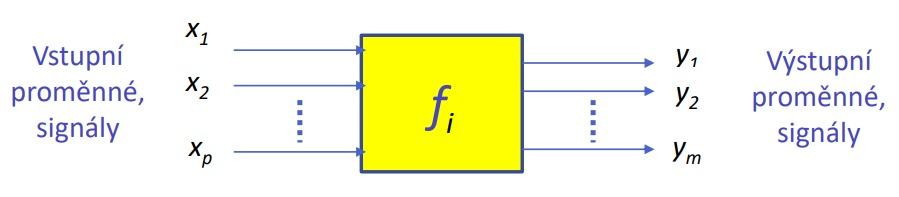
\includegraphics[width=0.7\linewidth]{img/SP-28_0.jpg}
	
	Logická funkce $y_k=f(x_1,x_2,x_3,...,x_p)$	existuje pro každý výstup y.
	
	\item možnosti reprezentace logických funkcí:
	\begin{itemize}
		\item tabulka
		
		\begin{tabular}{ |c|c| }
		\hline
		ab & f \\
		\hline
		00 & 0 \\
		01 & 1 \\
		10 & 1 \\
		11 & 0 \\
		\hline
		\end{tabular}
		
		\item n-rozměrná krychle
		
		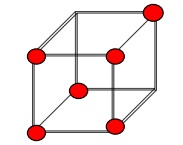
\includegraphics[width=0.2\linewidth]{img/SP-28_1.jpg}		
		
		\item Booleovský výraz
		
		Viz výše		
		
		\item mapa (Karnaughova)
		
		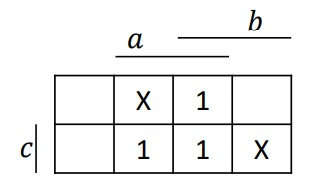
\includegraphics[width=0.25\linewidth]{img/SP-28_2.jpg}		
		
	\end{itemize}
	
	\item možnosti realizace obvodů:
	\begin{itemize}
		\item na úrovni hradel
		\item mapování na technologii (FPGA, ASIC)
		\item popis v jazyku (VHDL, Verilog)
	\end{itemize}
	
\end{itemize}

\subsubsection*{Sekvenční obvody}

\begin{itemize}
	\item výstup závisí na posloupnosti/sekvenci hodnot na vstupu
	\item zapamatování se realizuje zpětnou vazbou
	\item popsány konečným stavovým automatem
	\item typy sekvenčních obvodů:
	\begin{itemize}
		\item Moore
		 
		Obvod, jehož výstup závisí pouze na vnitřním stavu.
		
		\item Mealy
		
		Obvod, jehož výstup závisí také na aktuálním vstupu (kromě stavu).
	\end{itemize}
	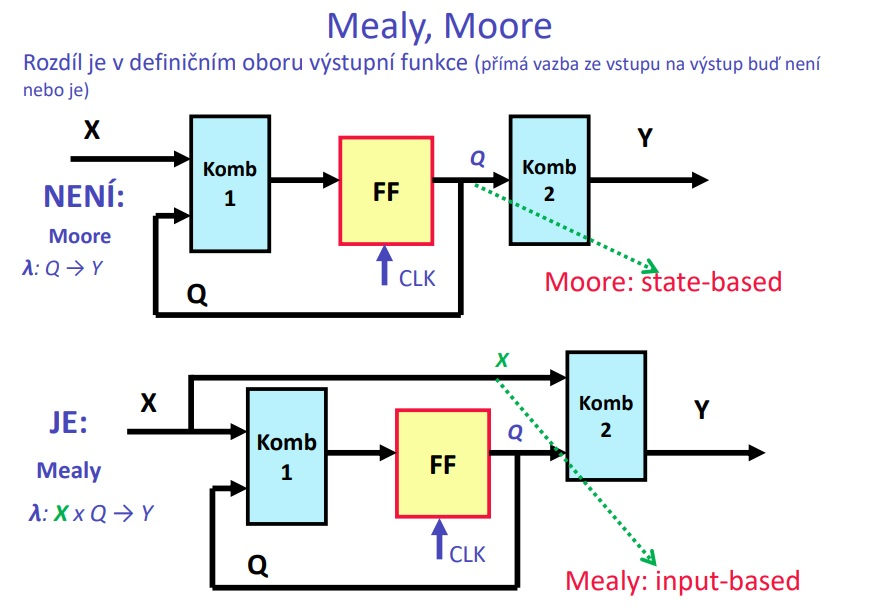
\includegraphics[width=0.6\linewidth]{img/SP-28_3.jpg}		
	
\end{itemize}

\subsubsection*{Implementace na úrovni hradel}
\begin{itemize}
	\item nejprve minimalizace logické funkce a zápis výsledku např. v Booleovském výrazu
	\item následně nakreslení/vytvoření funkce pomocí základních hradel --- NOT, AND, OR, NAND, NOR, XOR
\end{itemize}

\subsubsection*{Minimalizace logické funkce}
\begin{itemize}
	\item smysl --- zjednodušit a zkrátit zápis, snížit potřebný materiál pro výrobu
	\item minimalizace pomocí map --- založenana hledání co největších skupin sousedních stavů.
	\item postup při minimalizaci:
	\begin{itemize}
		\item vytvoření Karnaughovy mapy pro funkci
		\item nalezení všech přímých implikantů (maximální skupiny jedniček či "dont care")
		\item určení všech podstatných implikantů (obsahující jedničku, kterou jiný implikant neobsahuje)
		\item pokud nejsou pokryty všechny vrcholy s "1", nutno vybrat další přímé implikanty (takové, kde je nejméně negací)
	\end{itemize}
	
	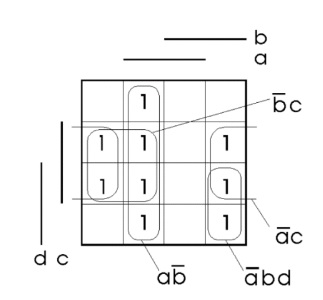
\includegraphics[width=0.4\linewidth]{img/SP-28_4.jpg}
	
	$a\overline{b}+\overline{b}c+\overline{a}c+\overline{a}bd$
	
	\item lze také kroužkovat nuly --- pak je ale nutné funkci sestavit jinak.
	
	$(\overline{a}+\overline{b})(a+c+d)(a+b+c)$
	
\end{itemize}

